\documentclass{../llncs/llncs}

% \input{src/new_preamble.tex}
%% The preamble
\usepackage[english]{babel} % Babel
\usepackage{import}

\usepackage[T1]{fontenc}
\usepackage[utf8]{inputenc}

\usepackage{underscore}
\usepackage{caption}


\usepackage{rotating}

% \usepackage{amssymb}
\usepackage{pifont}

\usepackage{wasysym}
\usepackage{bm}
\let\mathbf\relax

% \newcommand{\passmark}{\ding{51}}%
% \newcommand{\failmark}{\ding{55}}%
% \newcommand{\skipmark}{$\circ$}%
% \newcommand{\missmark}{$\bm{\circ}$}%
% \newcommand{\missmarkx}{$\bm{\ocircle}$}%

\usepackage{xcolor}
\definecolor{greeny}{RGB}{0,128, 0}
\definecolor{redy}{RGB}{255,0, 0}
\definecolor{bluey}{RGB}{0,0,255}
\newcommand{\passmark}{{\color{greeny}\ding{51}}}%
\newcommand{\failmark}{{\color{red}\ding{55}}}%
\newcommand{\skipmark}{{\color{blue}$\circ$}}%
\newcommand{\missmark}{$\bm{\circ}$}%
\newcommand{\missmarkx}{$\bm{\ocircle}$}%
% FIXME different way of naming the cards?
\newcommand{\Acard}{A\xspace} % A and A new merged together
\newcommand{\Bcard}{B\xspace}
\newcommand{\Ccard}{C\xspace}
\newcommand{\Cnewcard}{C*\xspace}
\newcommand{\Dcard}{D\xspace}
\newcommand{\Ecard}{E\xspace}
\newcommand{\Fcard}{F\xspace}
\newcommand{\Gcard}{G\xspace}
\newcommand{\Hcard}{H\xspace}
\newcommand{\Icard}{I\xspace}
\newcommand{\Inewcard}{I*\xspace}
\newcommand{\Jcard}{J\xspace}
\newcommand{\vulnscap}{\mintinline[breaklines,breakafter=.]{python}{vulns.new.cap}\xspace}
\newcommand{\vulnscaporig}{\mintinline[breaklines,breakafter=.]{python}{vulns.cap}\xspace}

\newcommand{\appletscap}{\mintinline[breaklines,breakafter=.]{python}{applets.cap}\xspace}
\newcommand{\transactionconfusioncap}{\mintinline[breaklines,breakafter=_]{python}{transaction_confusion.cap}\xspace}

\newcommand{\scardenottransacted}{\mintinline[breaklines,breakafter=_]{python}{SCARD_E_NOT_TRANSACTED}\xspace}
\newcommand{\scardwunpoweredcard}{\mintinline[breaklines,breakafter=_]{python}{SCARD_W_UNPOWERED_CARD}\xspace}
\newcommand{\scardwunresponsivecard}{\mintinline[breaklines,breakafter=_]{python}{SCARD_W_UNRESPONSIVE_CARD}\xspace}

\newcommand{\jerror}{\mintinline[breaklines,breakafter=_]{python}{0x6438}\xspace}

\newcommand*\rot{\rotatebox{90}}
% fixing labelling enum items
\usepackage{xparse}
\let\realItem\item % save a copy of the original item
\makeatletter
\NewDocumentCommand\myItem{ o }{%
   \IfNoValueTF{#1}%
      {\realItem}% add an item
      {\realItem[#1]\def\@currentlabel{#1}}% add an item and update label
}
\makeatother


\usepackage{enumitem}    
\setlist[enumerate]{
    before=\let\item\myItem,       % use \myItem in enumerate
    label=\textnormal{(\arabic*)}, % format the label
    % widest=(2')                    % set the widest label
}

\newcommand{\baloadbastore}{\mintinline[breaklines, breakafter=_]{python}{baload_bastore}\xspace}
\newcommand{\baload}{\mintinline[breaklines, breakafter=_]{python}{baload}\xspace}
\newcommand{\bastore}{\mintinline[breaklines, breakafter=_]{python}{bastore}\xspace}


\newcommand{\cla}{\mintinline{python}{CLA}\xspace}
\newcommand{\ins}{\mintinline{python}{INS}\xspace}
\newcommand{\pone}{\mintinline{python}{P1}\xspace}
\newcommand{\ptwo}{\mintinline{python}{P2}\xspace}
\newcommand{\lc}{\mintinline{python}{Lc}\xspace}
\newcommand{\data}{\mintinline{python}{Data}\xspace}
\newcommand{\len}{\mintinline{python}{Le}\xspace}

\newcommand{\getstatic}{\mintinline[breaklines, breakafter=_]{python}{getstatic_<T>}\xspace}
\newcommand{\putstatic}{\mintinline[breaklines, breakafter=_]{python}{putstatic_<T>}\xspace}

\newcommand{\getfield}{\mintinline[breaklines, breakafter=_]{python}{getfield_a}\xspace}

\newcommand{\prepareone}{\mintinline[breaklines,breakafter=_]{python}{INS_PREPARE1}\xspace}
\newcommand{\preparetwo}{\mintinline[breaklines,breakafter=_]{python}{INS_PREPARE2}\xspace}
\newcommand{\insreadmem}{\mintinline[breaklines,breakafter=_]{python}{INS_READMEM}\xspace}

\newcommand{\ping}{\mintinline[breaklines,breakafter=_]{python}{PING}\xspace}
\newcommand{\status}{\mintinline[breaklines,breakafter=_]{python}{STATUS}\xspace}
\newcommand{\setup}{\mintinline[breaklines,breakafter=_]{python}{SETUP}\xspace}
\newcommand{\readmem}{\mintinline[breaklines,breakafter=_]{python}{READ_MEM}\xspace}
\newcommand{\writemem}{\mintinline[breaklines, breakafter]{python}{WRITE_MEM}\xspace}
\newcommand{\cleanup}{\mintinline[breaklines,breakafter=_]{python}{CLEANUP}\xspace}

\newcommand{\triggerswapx}{\mintinline[breaklines,breakafter=_]{python}{TRIGGER_SWAPX}\xspace}

\newcommand{\nreadshort}{\mintinline[breaklines,breakafter=_]{python}{NREAD_SHORT}\xspace}
\newcommand{\nwriteshort}{\mintinline[breaklines,breakafter=_]{python}{NWRITE_SHORT}\xspace}

\newcommand{\getfieldins}{\mintinline[breaklines,breakafter=_]{python}{GETFIELD_<T>}\xspace}
\newcommand{\putfieldins}{\mintinline[breaklines,breakafter=_]{python}{PUTFIELD_<T>}\xspace}

\newcommand{\getstaticins}{\mintinline[breaklines,breakafter=_]{python}{GET_STATIC}\xspace}

\newcommand{\byte}{\mintinline[breaklines, breakafter=_]{python}{byte}\xspace}

\newcommand{\arraycopy}{\mintinline[breaklines, breakafter=_]{python}{arraycopy}\xspace}
\newcommand{\setShort}{\mintinline[breaklines, breakafter=_]{python}{setShort}\xspace}
\newcommand{\setInt}{\mintinline[breaklines, breakafter=_]{python}{setInt}\xspace}
\newcommand{\arrayFill}{\mintinline[breaklines, breakafter=_]{python}{arrayFill}\xspace}
\newcommand{\arrayFillNonAtomic}{\mintinline[breaklines, breakafter=_]{python}{arrayFillNonAtomic}\xspace}

\newcommand{\arrayCopy}{\mintinline[breaklines, breakafter=_]{python}{arrayCopy}\xspace}
\newcommand{\arrayCopyNonAtomic}{\mintinline[breaklines, breakafter=_]{python}{arrayCopyNonAtomic}\xspace}

\newcommand{\arrayops}{\mintinline[breaklines, breakafter=_]{python}{arrayops}\xspace}
\newcommand{\staticfieldref}{\mintinline[breaklines, breakafter=_]{python}{staticfield_ref}\xspace}
\newcommand{\referencelocation}{\mintinline[breaklines, breakafter=_]{python}{referencelocation}\xspace}
\newcommand{\swapx}{\mintinline[breaklines, breakafter=_]{python}{swap_x}\xspace}
\newcommand{\nativemethod}{\mintinline[breaklines, breakafter=_]{python}{nativemethod}\xspace}

% classes
\newcommand{\builderclass}{\mintinline[breaklines,breakafter=.,breakbefore=BA]{python}{javus.builder.BaseAttackBuilder}\xspace}
\newcommand{\shortbuilderclass}{\mintinline[breaklines,breakbefore=AB]{python}{BaseAttackBuilder}\xspace}
\newcommand{\attackbuilder}{\mintinline[breaklines,breakbefore=B]{python}{AttackBuilder}\xspace}

\newcommand{\executorclass}{\mintinline[breaklines,breakbefore=BE]{python}{javus.executor.BaseExecutorBuilder}\xspace}
\newcommand{\shortexecutorclass}{\mintinline[breaklines,breakbefore=BE]{python}{BaseExecutorBuilder}\xspace}
\newcommand{\attackexecutor}{\mintinline[breaklines,breakbefore=AB]{python}{AttackExecutor}\xspace}

\newcommand{\appclass}{\mintinline[breaklines,breakafter=.]{python}{javus.analyzer.App}\xspace}
\newcommand{\shortappclass}{\mintinline{python}{App}\xspace}

\usepackage{algpseudocode}
\usepackage{algorithm}
% \usepackage[ruled,vlined]{algorithm2e}

\usepackage{booktabs}

\usepackage{algorithm}
% \lstset{
%   mathescape = true,
%   basicstyle = \ttfamily}
% \newcommand{\dollar}{\mbox{\textdollar}}

% \lstdefinestyle{}
% {
    % numberblanklines=false,
    % language=shell,
    % tabsize=4,
    % keywordstyle=\color{red},
    % identifierstyle= %plain identifiers for make
% }

%\lstinputlisting[
%    inputencoding=latin1, 
%    firstline=1, 
%    %lastline=10,
%    caption={[Makefile]Makefile, foobar},
%    style=makefile
%]{./src/makefile}

\usepackage{svg}
\newcommand{\javusdev}{\mintinline{bash}{javusdev}\xspace}
\newcommand{\javus}{\mintinline{bash}{javus}\xspace}
\newcommand{\javusrun}{\mintinline{bash}{javus run}\xspace}
\newcommand{\javusweb}{\mintinline{bash}{javus web}\xspace}
\newcommand{\javuslist}{\mintinline{bash}{javus list}\xspace}
\newcommand{\javusvalidate}{\mintinline{bash}{javus validate}\xspace}
\newcommand{\jcmvanalysis}{\mintinline[breaklines,breakafter=-]{python}{javus}\xspace}
\newcommand{\ant}{\texttt{ant}\xspace}
\newcommand{\petr}{Petr Švenda\xspace}

\newcommand{\projectroot}{\mintinline[breaklines,breakafter=-]{python}{javus}\xspace}
\newcommand{\install}{\mintinline{bash}{install}\xspace}
\newcommand{\send}{\mintinline{bash}{send}\xspace}
\newcommand{\uninstall}{\mintinline{bash}{uninstall}\xspace}

\newcommand{\projectname}{JavaCard Vulnerability Scanner\xspace}

\newcommand{\scenario}{\mintinline{python}{Scenario}\xspace}

\newcommand{\stageinstall}{\mintinline{python}{_install}\xspace}
\newcommand{\stagesend}{\mintinline{python}{_send}\xspace}
\newcommand{\stageuninstall}{\mintinline{python}{_uninstall}\xspace}

\newcommand{\selectable}{\mintinline{python}{SELECT}able\xspace}

\newcommand{\examplemodule}{\mintinline[breaklines,breakafter=_]{python}{example_attack.py}\xspace}

% TODO publish the project and add the url!
% \newcommand{\gitlaburl}{\url{https://gitlab.com/quapka/javus}}
\newcommand{\githuburl}{https://github.com/quapka/javus.git}
% TODO fix the minted environements, see projects/sandbox/latex/mint-caption

\newcommand{\finalcommit}{TODO HASH OF THE FINAL COMMIT}

% \title{Talk proposal: Security analysis of JavaCard Virtual Machine}
\author{Anonymized}
\institute{Masaryk University, Faculty of Informatics, Brno}

\newcommand{\swappletselectfailed}{\mintinline[breaklines,breakafter=_]{python}{SW_APPLET_SELECT_FAILED (0x6999)}\xspace}
\newcommand{\shortswappletselectfailed}{\mintinline[breaklines,breakafter=_]{python}{SW_APPLET_SELECT_FAILED}\xspace}
\newcommand{\swbytesremaining}{\mintinline[breaklines,breakafter=_]{python}{SW_BYTES_REMAINING_00 (0x6100)}\xspace}
\newcommand{\shortswbytesremaining}{\mintinline[breaklines,breakafter=_]{python}{SW_BYTES_REMAINING_00}\xspace}
\newcommand{\swclanotsupported}{\mintinline[breaklines,breakafter=_]{python}{SW_CLA_NOT_SUPPORTED (0x6E00)}\xspace}
\newcommand{\shortswclanotsupported}{\mintinline[breaklines,breakafter=_]{python}{SW_CLA_NOT_SUPPORTED}\xspace}
\newcommand{\swcommandchainingnotsupported}{\mintinline[breaklines,breakafter=_]{python}{SW_COMMAND_CHAINING_NOT_SUPPORTED (0x6884)}\xspace}
\newcommand{\shortswcommandchainingnotsupported}{\mintinline[breaklines,breakafter=_]{python}{SW_COMMAND_CHAINING_NOT_SUPPORTED}\xspace}
\newcommand{\swcommandnotallowed}{\mintinline[breaklines,breakafter=_]{python}{SW_COMMAND_NOT_ALLOWED (0x6986)}\xspace}
\newcommand{\shortswcommandnotallowed}{\mintinline[breaklines,breakafter=_]{python}{SW_COMMAND_NOT_ALLOWED}\xspace}
\newcommand{\swconditionsnotsatisfied}{\mintinline[breaklines,breakafter=_]{python}{SW_CONDITIONS_NOT_SATISFIED (0x6985)}\xspace}
\newcommand{\shortswconditionsnotsatisfied}{\mintinline[breaklines,breakafter=_]{python}{SW_CONDITIONS_NOT_SATISFIED}\xspace}
\newcommand{\swcorrectlength}{\mintinline[breaklines,breakafter=_]{python}{SW_CORRECT_LENGTH_00 (0x6C00)}\xspace}
\newcommand{\shortswcorrectlength}{\mintinline[breaklines,breakafter=_]{python}{SW_CORRECT_LENGTH_00}\xspace}
\newcommand{\swdatainvalid}{\mintinline[breaklines,breakafter=_]{python}{SW_DATA_INVALID (0x6984)}\xspace}
\newcommand{\shortswdatainvalid}{\mintinline[breaklines,breakafter=_]{python}{SW_DATA_INVALID}\xspace}
\newcommand{\swfilefull}{\mintinline[breaklines,breakafter=_]{python}{SW_FILE_FULL (0x6A84)}\xspace}
\newcommand{\shortswfilefull}{\mintinline[breaklines,breakafter=_]{python}{SW_FILE_FULL}\xspace}
\newcommand{\swfileinvalid}{\mintinline[breaklines,breakafter=_]{python}{SW_FILE_INVALID (0x6983)}\xspace}
\newcommand{\shortswfileinvalid}{\mintinline[breaklines,breakafter=_]{python}{SW_FILE_INVALID}\xspace}
\newcommand{\swfilenotfound}{\mintinline[breaklines,breakafter=_]{python}{SW_FILE_NOT_FOUND (0x6A82)}\xspace}
\newcommand{\shortswfilenotfound}{\mintinline[breaklines,breakafter=_]{python}{SW_FILE_NOT_FOUND}\xspace}
\newcommand{\swfuncnotsupported}{\mintinline[breaklines,breakafter=_]{python}{SW_FUNC_NOT_SUPPORTED (0x6A81)}\xspace}
\newcommand{\shortswfuncnotsupported}{\mintinline[breaklines,breakafter=_]{python}{SW_FUNC_NOT_SUPPORTED}\xspace}
\newcommand{\swincorrectpp}{\mintinline[breaklines,breakafter=_]{python}{SW_INCORRECT_P1P2 (0x6A86)}\xspace}
\newcommand{\shortswincorrectpp}{\mintinline[breaklines,breakafter=_]{python}{SW_INCORRECT_P1P2}\xspace}
\newcommand{\swinsnotsupported}{\mintinline[breaklines,breakafter=_]{python}{SW_INS_NOT_SUPPORTED (0x6D00)}\xspace}
\newcommand{\shortswinsnotsupported}{\mintinline[breaklines,breakafter=_]{python}{SW_INS_NOT_SUPPORTED}\xspace}
\newcommand{\swlastcommandexpected}{\mintinline[breaklines,breakafter=_]{python}{SW_LAST_COMMAND_EXPECTED (0x6883)}\xspace}
\newcommand{\shortswlastcommandexpected}{\mintinline[breaklines,breakafter=_]{python}{SW_LAST_COMMAND_EXPECTED}\xspace}
\newcommand{\swlogicalchannelnotsupported}{\mintinline[breaklines,breakafter=_]{python}{SW_LOGICAL_CHANNEL_NOT_SUPPORTED (0x6881)}\xspace}
\newcommand{\shortswlogicalchannelnotsupported}{\mintinline[breaklines,breakafter=_]{python}{SW_LOGICAL_CHANNEL_NOT_SUPPORTED}\xspace}
\newcommand{\swnoerror}{\mintinline[breaklines,breakafter=_]{python}{SW_NO_ERROR (0x9000)}\xspace}
\newcommand{\shortswnoerror}{\mintinline[breaklines,breakafter=_]{python}{SW_NO_ERROR}\xspace}
\newcommand{\swrecordnotfound}{\mintinline[breaklines,breakafter=_]{python}{SW_RECORD_NOT_FOUND (0x6A83)}\xspace}
\newcommand{\shortswrecordnotfound}{\mintinline[breaklines,breakafter=_]{python}{SW_RECORD_NOT_FOUND}\xspace}
\newcommand{\swsecuremessagingnotsupported}{\mintinline[breaklines,breakafter=_]{python}{SW_SECURE_MESSAGING_NOT_SUPPORTED (0x6882)}\xspace}
\newcommand{\shortswsecuremessagingnotsupported}{\mintinline[breaklines,breakafter=_]{python}{SW_SECURE_MESSAGING_NOT_SUPPORTED}\xspace}
\newcommand{\swsecuritystatusnotsatisfied}{\mintinline[breaklines,breakafter=_]{python}{SW_SECURITY_STATUS_NOT_SATISFIED (0x6982)}\xspace}
\newcommand{\shortswsecuritystatusnotsatisfied}{\mintinline[breaklines,breakafter=_]{python}{SW_SECURITY_STATUS_NOT_SATISFIED}\xspace}
\newcommand{\swunknown}{\mintinline[breaklines,breakafter=_]{python}{SW_UNKNOWN (0x6F00)}\xspace}
\newcommand{\shortswunknown}{\mintinline[breaklines,breakafter=_]{python}{SW_UNKNOWN}\xspace}
\newcommand{\swwarningstateunchanged}{\mintinline[breaklines,breakafter=_]{python}{SW_WARNING_STATE_UNCHANGED (0x6200)}\xspace}
\newcommand{\shortswwarningstateunchanged}{\mintinline[breaklines,breakafter=_]{python}{SW_WARNING_STATE_UNCHANGED}\xspace}
\newcommand{\swwrongdata}{\mintinline[breaklines,breakafter=_]{python}{SW_WRONG_DATA (0x6A80)}\xspace}
\newcommand{\shortswwrongdata}{\mintinline[breaklines,breakafter=_]{python}{SW_WRONG_DATA}\xspace}
\newcommand{\swwronglength}{\mintinline[breaklines,breakafter=_]{python}{SW_WRONG_LENGTH (0x6700)}\xspace}
\newcommand{\shortswwronglength}{\mintinline[breaklines,breakafter=_]{python}{SW_WRONG_LENGTH}\xspace}
\newcommand{\swwrongpp}{\mintinline[breaklines,breakafter=_]{python}{SW_WRONG_P1P2 (0x6B00)}\xspace}
\newcommand{\shortswwrongpp}{\mintinline[breaklines,breakafter=_]{python}{SW_WRONG_P1P2}\xspace}


% \usepackage{listing}
\usepackage[outputdir=build]{minted}
\newcommand{\filepath}[1]{\mintinline[breakanywhere,breaklines=true,breakafter=./-]{python}{#1}}
\newcommand{\class}[1]{\mintinline[breakanywhere,breaklines=true,breakafter=.]{python}{#1}}

\newcommand{\constantstaticfieldref}{\mintinline[breaklines,breakafter=_]{python}{CONSTANT_StaticFieldref_info.offset}\xspace}

% break lines in \mintinline commands
% \setmintedinline{breakafter=.}

% \newcommand{\PYZdl}{\textdollar}
\usepackage{xspace}

% TODO how to typeset undescores!

\hyphenation{APDU}
\hyphenation{APDUs}

\hyphenation{SDK}
\hyphenation{SDKs}

\hyphenation{CAP}
\hyphenation{CAPs}

% \newcommand{\unsuccessful}{(un)suc\discretionary{-}{}cessful}
\hyphenation{suc-cess-ful}
\hyphenation{sta-ges}

\hyphenation{Java-Card}
\hyphenation{Java-Cards}
\hyphenation{app-let}
\hyphenation{Un-for-tu-na-te-ly}
\hyphenation{au-to-ma-ti-ca-lly}

\hyphenation{straight-for-ward}

% \setlength{\tabcolsep}{20pt}
% \renewcommand{\arraystretch}{1.5}

\newlength{\oldtabcolsep}
\setlength{\oldtabcolsep}{\tabcolsep}

\newlength{\oldfloatsep}
\setlength{\oldfloatsep}{\floatsep}
% \newlength{\oldarraystretch}
% \setlength{\oldarraystretch}{\arraystretch}
% \setlength{\parindent}{2em}

% \oldtabcolsep{\tabcolsep}
% \oldarraystretch{\arraystretch}
% \setlength{\myparindent}{\parindent}
% \setlength{\parindent}{2em}

%restore original
% \setlength{\parindent}{\myparindent}


% metadata information
\title{Talk proposal: Security analysis of JavaCard Virtual Machine}
\author{Anonymized}
\institute{Masaryk University, Faculty of Informatics, Brno}


\begin{document}
\maketitle

\begin{abstract}
    % FIXME simplify
This text investigates the state of the art security of JavaCards. Firstly, the JavaCard platform and its defensive mechanisms are described. Secondly, the author introduces few existing attacks against the JavaCard platform. Furthermore, the author remarks that with rising number of attacks it is increasingly more difficult to systematically test a real JavaCard against all of them and assess the level of security of the JavaCard. Then the design of a new tool JavaCard Vulnerability Scanner created by the author is introduced, which presents a possible solution to the previous situation. This tool can automatically test the security of a real JavaCard against several of the previously presented attacks, moreover it is also extensible with other attacks in the future. Finally, results from the execution of JavaCard Vulnerability Scanner on several JavaCards are discussed.
\keywords{JavaCard security analysis \and smartcard \and JavaCard Vulnerability Scanner \and \texttt{javus}}
\end{abstract}


% \import{src/sections/}{sec1-opening-section.tex}

\section{Introduction}

This text was created to propose a talk for the Keymaker track at SantaCrypt2020\footnote{Czech and Slovak crypto related conference, see \url{https://mkb.tns.cz/cfp.htm}.}. Let us hope that the current circumstances will allow it to happen. This text follows the structure of the master's thesis Security analysis of JavaCard Virtual Machine~\cite{anon2020thesis} defended by the author in September 2020. The text is mostly comprised of excerpts from the thesis. The reader is welcomed to read the thesis if he or she wishes to get more in-depth discussion of the following topics.
% The section~\ref{sec:fuzzing} is explained in a little bit more detail in here than in the original thesis.
% TODO introduce each section

\section{State of the art of JavaCard security\label{sec:state-of-the-art}}
JavaCard technology is based on the Java programming language and allows programs created in Java to be executed on secure devices such as smartcards. Similarly to Java, JavaCard system is made up from multiple components such as JavaCard Virtual Machine (JCVM), JavaCard Runtime Environment (JCRE), JavaCard Application Programming Interface (JCAPI) and additionally JavaCard Convertor (JCC).  Smartcards are pocket sized devices with an embedded microchip. Smartcard's chip contains components such as CPU, RAM and ROM and non-volatile memory, known from other computing devices. However, the components inside a smartcard chip are much more limited in their capabilities. Typical size of a user RAM is around 12K. The size of non-volatile memory (that is a memory, that allows persistant data storage) is higher at around 16K and ROM is the biggest with 32-48K. Also, the computing power of a CPU inside a smartcard is nowhere near the computing power of CPUs used in computers.

JavaCard technology is released in multiple versions. The newest one at the time of writing this text is the version 3.1. The JavaCard platform specifications can be accessed at~\cite{jcspecs31download}.
%Since the version 3.0 JavaCard platform was split into Classic and Connected editions. The Connected edition targets devices that have restricted resources, but are more powerful than conventional smartcards described above. If we refer in our work to a version of JavaCard Platform higher than 3.0 we will mean the Classid Edition.

% In our work we focus only on the Classic edition for the version 3.0 and newer of JavaCard technology.

Each JavaCard technology version is accompanied with a corresponding JavaCard Software Development Kit (SDK).
% SDK equips JavaCard developers with the tools needed for the development of JavaCard programs.
In the context of JavaCard platform the programs are called JavaCard applets. As we will show later in the text, the behaviour of an particular applet with respect to security can differ across the SDKs and smartcards it is installed on.
% Because JavaCards are not that powerful, they cannot make use of all the features of the Java programming langugage. For that reason, only a subset of Java is used for developing JavaCard programs.
% Specifically, the JCVM supports only a subset of Java Virtual Machine. For example, JCVM does not support Security Manager class, threads or variable-length arguments. Furthermore, only some Java data types, like \texttt{boolean}, \texttt{byte}, \texttt{short}, \texttt{int} and Objects or arrays, are supported --- this implies that several bytecode instructions for handling more complicated types are not supported (the complete subset is described in~\cite{jcspecs31download}).

    \subsection{Applet lifetime}
% JavaCard applets are developed in the Java programming language.
The applet source files can define one or more Java packages. A package is referred to as an applet package if it contains a subclass of \class{javacard.framework.Applet} (there can be more than one). It is called a library package otherwise.  Similarly to Java, the source code is compiled into class files using Java compiler.
% The class files produced can now be tested and debugged.

Before the applet is downloaded to the target device the class files need to be converted using the JCC to a CAP (Converted APplet) file.

The CAP file format is the off-card representation of JavaCard application and can contain one or more applet and library packages. The CAP files consist of several different CAP components. JavaCard Converter produces a ``CAP file'' (it uses the \texttt{.cap} file extension), but it is actually a Java Archive file (JAR) that comprises of the individual CAP components. Some of the CAP components are required and some are optional.

The second input to the JCC after the class files are export files (EXP). Export files contain the name and linking information about the packages that are imported in the applet's source code.
Apart from creating CAP files JCC can also create export files for future conversions or JavaCard Assembly (JCA) files. JCA is human-readable version of the applet's bytecode.

Before the CAP file is downloaded to the target device an off-card verifier can be utilized to verify whether the file conforms to the specifications for a given SDK version. To load a converted CAP file onto a smartcard we need a Card Acceptance Device (CAD; smartcard reader).

Once a JavaCard is inserted into a reader we can use an installation tool to load the CAP file onto the device. The smartcard itself has an installation program, which needs to follow the specifications in~\cite{jcspecs31download}.
% FIXME the surroungding paragraphes!!

There are three steps that need to take place before the new applet can be used. The applet's CAP file needs to be loaded on the target device, than linked and finally the applets \mintinline{bash}{install(byte[], short, byte)} method is invoked (if the \texttt{install} method is not implemented then applet's objects cannot be created and initialized~\cite{jcspecs31download}). After the installation JavaCard RE interacts with the applet mostly through the methods \texttt{select}, \texttt{process}, \texttt{deselect}, \texttt{uninstall}.

% After all three steps proceed successfuly the applet is ready and can be used. In case of successful installation of an applet packgage the applet is made

Applets and packages are identified on card by their Application Identifier (AID) defined in ISO 7816-5~\cite{jcspecs31download}.
% AID value is concatenated from Registered Application Provider Identifier (RID) and Proprietary Application Identifier Extension (PIX)~\cite{globalplatform}.
The communication with the applet is facilitated through Application Protocol Data Unit (APDU). 
% The layout of general APDU command and response is in the table~\ref{tab:apdu}.

% \begin{table}
%     % \begin{tabular}{lc}
%         % \begin{minipage}{.5\linewidth}
%         \hfill
%         \parbox{.45\linewidth}{
%         \centering
%             \begin{tabular}{@{}lllllll@{}}
%                 \toprule
%                    \cla & \ins & \pone & \ptwo & \lc & \data & \len \\
%                 \midrule
%                    1 & 1 & 1& 1& 1 & 00--\lc& 0--3 \\
%                 \bottomrule
%             \end{tabular}
%             }
%         % \end{minipage} &
%         % \begin{minipage}{.5\linewidth}
%         \hfill
%         \parbox{.45\linewidth}{
%         \centering
%         \begin{tabular}{@{}lll@{}}
%             \toprule
%                 \data & \texttt{SW1} & \texttt{SW2}\footnotemark \\
%             \midrule
%                 max \len & 1 & 1 \\
%             \bottomrule
%         \end{tabular}
%         }
%         % \end{minipage}
%         \caption{The general structure of APDU command on the left and APDU response on right~\cite{jcspecs31download}. The field names are in the top row and their length in the bottom one.}
%         \label{tab:apdu}
%     % \end{tabular}
% \end{table}

% \footnotetext{\texttt{SW1SW2} are called status word. The values of status words are defined in the \texttt{javacard.framework.ISO7816} package.}

When CAD wants to interact with a particular applet, it issues a special APDU containing the applet's AID. JavaCard RE deselects (suspends) the currently selected applet by calling its \texttt{deselect} method and calls the \texttt{select} method of the applet that matches the AID. Further APDU payloads are then relayed to the applet through its \texttt{process} method. Finally, the \texttt{uninstall} method is called when a APDU requesting deletion of the applet is received by JCRE.

    % The \cla field from~\ref{tab:apdu} is used to differentiate higher level functionality of the applet. The \ins field is used to trigger particular operation in the applet. The \texttt{process} method usually implementes a \texttt{switch} statement that dispatches the \ins instructions to the respective methods. We will see the \ins field be used for communicating with the applets in POCs.

    \subsection{Attack models and defensive mechanisms}
    % As we will see in the list of related work~\ref{sec:related-work}, t
    The previous research distinguishes three main attack categories --- physical attacks, logical attacks and combined attacks. Physical attacks target the device physical components, such as CPU and memory, by for example shooting a laser beam at them. In~\cite{Prpic2010thesis} the power traces caused by the power consumption due to the execution of the bytecode instructions are stored and analyzed (for the purpose of reverse engineering in the future).
    % A database of such traces can then be used to partially reverse engineer the instruction in future interception of power traces of unknown code execution.
    Logical attacks like~\cite{hogenboom} target the software implementation of JavaCards and try to exploit bugs in the implementation of JCRE and JCVM (or even the card OS). Combined attacks combine the previous two.
    %Physical disturbance might allow skipping an internal validation of malicious applet, which would otherwise be prevented from execution as in~\cite{barbusecond}.

    % FIXME move elsewhere!!
    % \subsection{The attacker model}

        % Because we are interested in attacks on the JavaCard platform we need to discuss the attacker model first.
        % In general, the attacker model for the various attacks on JavaCards can differ.
        For physical attacks the attacker usually needs to have the target JavaCard in a long-term possession and may or may not need to be able to install additional applications on the JavaCard and to communicate with the card. For logical attacks, the attacker often needs to be able to install additional applications on the target device and then communicate with it (in rare cases this might not require physical access to the JavaCard as demonstrated in~\cite{se:gemalto:part2}). For combined attacks (the combination of the two previous) the adversary will probably need both the long-term access to the card and ability to install applets on it.
        % In the second section we present the JavaCard Vulnerability Scanner; this tool currently supports multiple logical attacks and for each one of them the attacker model is the same. The adversary needs to be in the possession of the target JavaCard, have the ability to install additional applets and issue APDU commands to it afterwards.

        JavaCard technology is build to be used in secure elements such as smartcards. Therefore it is natural that several defensive mechanisms are in place to attempt to stop the attacker from misusing the device and obtain information, that must be kept secret (e.g. private keys).
The techniques we are about to describe are software based. However, smartcards need also to be tamper resistant, because several destructive or invasive techniques can be utilized to compromise its security as showed in~\cite{kommerling}.
        % Smart cards in general are developed to be used in situation, where security is an important if not the most important requirement. They are used in banking industry, person identification (national ID cards, passports)  or for example as access tokens to buildings. Due to those reasons it is obvious, that mechanisms defending the secret information (such as private keys used in Public Key Infrastructures) stored on those cards need to defended well against various attack vectors.

% \section{Defensive Measures Against the Attacks}
    % \subsection{The Compiler}

% The Java compiler is used to compile the JavaCard source files into the class files. 
    \subsubsection{The off-card bytecode verifier}

% FIXME cite SDK
The various JavaCard SDKs are equiped with tools used for off-card verification of the CAP, EXP and JCA files~\cite{jcoffcardverifier}. After the CAP file conversion the off-card verification can take place. The internal integrity of the CAP file and the associated export files is verified according to the JCVM specifications~\cite{jcspecs31download}.

    \subsubsection{The on-card bytecode verifier}

    If the off-card bytecode verification is not enforced a malicious CAP file can be created and loaded onto a card. It is then up to the card to decide, whether it will accept or reject such CAP file. As we will see in the section~\ref{chp:results} the behaviour of JavaCards differs. Similarly, discrepanies in the implementation of on-card installer and JavaCard RE are observed in~\cite{lanettrojan}. The on-card bytecode verification is mandatory for JavaCard 3.0 Connected Edition and higher~\cite{barbusecond}. As observed in the previous results and in our own, it is apparent that JavaCard manufacturers implement the on-card bytecode verifier differently.
    % The verification happens while the CAP file is loaded.
    The verification can comprise of checking that the different CAP file components are present and the references to export files are resolved properly to the objects on the card.


    \subsubsection{Applet firewall}

    JavaCard technology allows multiple applications to be installed alongside on a single devices~\cite{jcspecs31download}. To prevent the different applets to accidentaly (or maliciously) access data of other applications the JCRE introduces in Applet firewall~\cite{jcspecs31download}. Different applets on JavaCard are assigned different memory regions called contexts. The firewall acts as a boundary between those contexts. Each CAP file of an applet package is assigned its own context, library packages share the context of the creating applet instance. One CAP file can define multiple applets --- those will share the same contexts and can therefore access objects of each other. Applets from one context are denied by the firewall access to applets from a different context.
    There is one special context assigned to the JavaCard RE. It possesses higher privileges and can access contexts of other applets.
    %Sometimes the applets from different contexts do need to access objects that reside in different context. Theses cases are covered by the following mechanisms --- JCRE Entry Points Objects, Sharing Arrays, JCRE privileges, Shareable Interfaces. An example of JCRE Entry Point Object is the APDU object that implments the buffer used for I/O operations with the CAD.


    \subsection{Existing logical attacks}
    In our research we are interested in the logical attacks exclusively. We will present few of the previously published attacks. For more exhaustive list of the existing logical attacks see~\cite{anon2020thesis,sergei,se:oracle:part1,se:oracle:part2,se:oracle:part3}.

    In his master's thesis~\cite{sergei} Sergei Volokitin presents several attacks against JavaCards.
    % ~\cite{sergei} describes maltitude of attacks.
    The most interesting ones are attacks on the secure containers such as \texttt{OwnerPIN}. The author first finds the object in memory, which is stored encrypted, then uses chosen plaintext cryptanalysis to learn that the PIN is encrypted using ECB mode. The author further noticies similarities in the handling of \texttt{OwnerPIN} and \texttt{DESKey} objects and finds out, that the \texttt{OwnerPIN} can by decrypted easily. Firstly, encrypted bytes of \texttt{OwnerPIN} are copied into a \texttt{DESKey} controlled by the attacker, then \texttt{getKey} method is called on the unsuspecting \texttt{DESKey} and the \texttt{PIN} is retrieved to the attacker.

    \subsubsection{Security Explorations}\label{subsec:security-explorations}

    In 2019 a company from Poland called Security Explorations\footnotemark\ released five notices~\cite{se:oracle:part1,se:oracle:part2,se:oracle:part3,se:gemalto:part1,se:gemalto:part2} that describe security vulnerabilities in JavaCards. Overall, they have reported 34 individual issues. The reports~\cite{se:oracle:part1,se:oracle:part2,se:oracle:part3} test the vulnerabilities on JavaCard Reference Implementation from Oracle~\cite{jcspecs31download}  and cover issues like insufficient implementation of JCVM bytecode instructions and JCAPI methods or handling of CAP file and its insufficient verification. The individual issues have been verified by Security Explorations on the Reference implementation (the Reference implementation binary is called \cref) of JavaCard technology version 3.1 (currently available for download at~\cite{jcspecs31download}).

The second batch of reports~\cite{se:gemalto:part1,se:gemalto:part2} analyze Gemalto JavaCard based products and identify vulnerabilities in the SIM Toolkit applet (STK applet). Those vulnerabilities are caused by unmanaged or leaking memory references. Most notable is the result in~\cite{se:gemalto:part2}, where the authors used the discovered vulnerability to load JavaCard applet over-the-air to a target SIM card. Furthermore, they conclude that it should be possible to exploit the vulnerabilities from~\cite{se:gemalto:part1,se:gemalto:part2} in such a way, that a hidden backdoor is loaded onto a SIM card.


\footnotetext{The company has seized to exist, however, its lead security researcher Adam Gowdiak is now working under Adam Gowdiak Security Research (see \url{http://www.agsecurityresearch.com/}).}

    The vulnerability noticies~\cite{se:oracle:part1,se:oracle:part2,se:oracle:part3} are also accompanied by a POC~\cite{se:downloadpage}, that help to demonstrate the issues. The POCs comprise of Java source files, custom Gen Tool and several batch scripts.


We will go through two of the POCs exploiting the vulnerabilites in~\cite{se:oracle:part1,se:oracle:part2,se:oracle:part3} in greater detail, however, all of them are included in \projectname. Each POC consists of two applets \appletscap and \vulnscaporig (from which a malicious \vulnscap is generated with the Gen Tool). Every POC then defines several instructions that are used to exploit the particular vulnerability.

% There aren't as many POCs as there are vulnerabilities discovered, because the POCs unite the vulnerabilities of similar nature. We will use the issue numbering as in the original reports. The following sections briefly describe the vulnerabilities from~\cite{se:oracle:part1}.

\subsubsection{POC \texttt{arraycopy}}\label{subsec:arraycopy-explanation}
The JCAPI methods \arrayCopy and \arrayCopyNonAtomic from \mintinline[breaklines,breakafter=.]{python}{javacard.framework.Util} class~\cite{jcspecs31download} do not perform sufficient checks on input arguments. Both methods fail to prevent passing object instance (instead of an array) as an input argument. \cite{se:oracle:part1} mentions, that some similar methods do the input validation properly. The POC implements the instructions \readmem and \writemem, that can read and write memory through exploitation of one of the aforementioned methods.

% \subsubsection{POC \texttt{arrayops}}
% As was explained in~\ref{subsec:arraycopy-explanation}, it is not always the case, that array methods perform sufficient validation of the its arguments. A custom crafted object can be passed as an input argument instead of an array reference. Such object is then interpreted as an array of a very large size. The POC \arrayops exploits the methods \arrayFill, \arrayFillNonAtomic, \setShort, \setInt. The POC applet defines two instructions \readmem and \writemem, that allow to read and write outside of the allowed memory regions.

% \subsection{POC \texttt{baload_bastore}}
% The bytecode instructions \baload and \bastore load byte or boolean from array, respectively store byte or boolean from array~\cite{jcspecs31download}. The array argument to \baload instruction is checked and Security Exception is raised if the array is an array of shorts, integers or objects. Otherwise, the execution proceeds. However, instead of an array the argument can be a single object and the checks pass as well. 
% The POC code defines six different instructions --- \ping, \status, \setup are used to check and setup the vulnerability state. The instructions \readmem and \writemem demonstrate reading and writing memory. Final instruction \cleanup is used to clean the initial exploit setup. The~\cite{se:oracle:part1} state the impact of the vulnerability is ``compromise of memory safety / arbitrary read access to card memory''.

% \subsection{POC \texttt{nativemethod}}
% The \texttt{Method} CAP file component is used to describe methods, that are defined within the CAP file. The \mintinline[breaklines,breakafter]{python}{method_info.method_header_info} specify whether the method is native or not. The values in the field \texttt{method_header_info} can be changed and make this method a native one. This approach can be used to call native methods such as~\texttt{readByte}, \texttt{readShort}, \texttt{writeByte} and \texttt{writeShort}, that should be inaccessible to the current class.
% The POC implements two instructions \nreadshort and \nwriteshort, that invoke the native methods \texttt{readShort} and \texttt{writeShort}, respectively. A short value can be read or written with those instructions, that would be otherwise inaccessible.


% \subsection{POC \texttt{referencelocation}}
% Some bytecode instructions, like \getfield reference various fields and methods. Those references are stored as indeceses to the Constant Pool (\mintinline{python}{ConstantPool} CAP component), that contains tokens for the fields and methods at each index. The internal representation of those tokens is substituted for the indeces when a CAP file is loaded on JavaCard.~\cite{se:oracle:part1} refers to this process as ``linking''. The \texttt{ReferenceLocation} component stores the table of locations for each of the previously described substitutions.
% Before, the ``linking'' is done, each token value is checked to assure, that its value does not go beyond the size for the object (recall, that the token values refer to object fields and methods). If the value overflows, it is trimmed. However, if an entry in the \texttt{ReferenceLocation} table is omitted, the corresponding check of the token value is skipped as well, thus allowing the \getfield instruction access beyond the object size.
% The POC defines six instructions \getfieldins, \putfieldins\footnotemark, which allow to read and write the memory through a custom token value. 
% \footnotetext{The \texttt{<T>} refers to the particular type of the underlying bytecode instruction defined in~\cite{jcspecs31download}.}

% \subsection{POC \texttt{staticfieldref}}
% As explained in~\ref{sec:jc:lifecycle} CAP file comprises of different CAP components one of which is \mintinline{python}{StaticField} component. This component is referenced through \constantstaticfieldref item~\cite{jcspecs31download}. The \texttt{offset} value is not checked and can be changed, to point to arbitrary value. Then, through the use of byte instructions \getstatic\footnotemark and \putstatic the memory at the new \texttt{offset} can be read and written, respectively. The POC uses single instruction~\getstaticins, that returns the \texttt{offset} value, that was maliciously altered after the POC CAP file conversion.
% \footnotetext{Both \getstatic and \putstatic represent several bytecode instructions for particular types.}

\subsubsection{POC \texttt{swap_x}}
JCVM is stack based and uses frames to hold the information about the currently executed method, such as local variables and the operand stack. The bytecode instruction \swapx allows to swap $M$ words with $N$ words, that reside in the operand stack directly below. The intention is to swap one or two words on the stack~\cite{jcspecs31download}. If larger values for $N$ are provided a potential return address or instruction override can happen.
The POC code has a single instruction \triggerswapx, that invokes the malformed \swapx instruction. According to~\cite{se:oracle:part1} the instruction is expected to return \mintinline{python}{0x1234}, however, when executed in JCRE for \texttt{cref} a crash is observed in~\cite{se:oracle:part1} instead. When we have tested this POC on real JavaCards we have received the expected response
% as is discussed in~\ref{subsec:swapx}
on four of them as showed in the table~\ref{tab:best-swap_x}.


\subsubsection{Related JavaCard testing tools}
Riscure, a Dutch company located in Delft, has a product called JCworkBench, that can be used to perform a robust security of a real JavaCard as demonstrated in~\cite{jcworkbench,riscurejcworkbenchpdf}. However, it is not clear from Riscure's website~\cite{riscureweb}, whether it can still be purchased as it is not listed there anywhere.\footnotemark

\footnotetext{The tool was only found presumably for sale on a different website at \url{https://www.etesters.com/product/7E9C25F0-D8CC-0B99-67BC-8BF36D42FE30/smart-card-security-test-tool/}}

JavaCard Firewall Tester briefly introduced in~\cite{Mostowski07testingthe} is no longer available for download at~\cite{firewalltester} and the download site does not seem to be maintained anymore.

Two notable JavaCard testing tools are JCAlgTest~\cite{jcalgtest} and\linebreak ECTester~\cite{ectester}, both developed at CRoCS~\cite{crocsweb}. However, both those tools assess the security and safety of the implementation of the cryptograhical primitives and algorithms and not the resistance of JCRE or JCVM to logical attacks.

\section{JavaCard Vulnerability Scanner}\label{sec:javacard-vulnerability-scanner}
Naturally, a question arises: Is there even a need for a tool, that would test the shortcomings of JavaCard VM and JavaCard RE?  In the last section we have mentioned previous research, some of which includes the source code for a POC attack. However, if the reader imagines himself holding a JavaCard and wondering, whether it is vulnerable to a specific kind of an attack there is still \textit{a lot} of work to be done. Some of the POCs are \textit{only} included in the original paper and not accompanied with the source and build files. Or in the case of vulnerabilities discovered by Security Explorations the source code is included (as a ZIP archive), but the attacks are automated only for use with the reference implementation of JCRE.
% Also, they are built only with SDK 3.0.5GA. Given the number of new attacks discovered in the last years~\cite{se:oracle:part1, se:oracle:part2, se:oracle:part3, se:gemalto:part1, se:gemalto:part2} it is increasingly harder to perform systematic security analysis of a real JavaCard against all known (logical) attacks.

    The work done in author's thesis~\cite{anon2020thesis} resulted in an automated testing tool called \projectname. The thesis explains its architecture, design choices and usage in much more detail. Here we will only present the most important points.
    
    \subsection{The design of the testing framework}
% First, we will start with the list of the specifications for the framework. Before we go through them one by one and look at the way that they are implemented in more detail we define some terms and explain the project structure.

% \subsection{The framework specifications}
    We will start by laying down the specifications for the implementation of \projectname:
    \begin{enumerate}
        \item execute registered logical attacks on a real physical JavaCard % (see~\ref{sec:build-execute-attacks}),
        \item visualize the results of the attacks in a concise and clear manner % (see~\ref{sec:visualization}),
        \item be extensible --- allow adding new attacks in the future % (see~\ref{sec:attack-recipe}).
        \item be cross-platform, i.e. support at least Linux and Windows platforms % (see~\ref{sec:invocation}),
    \end{enumerate}


    And we also introduce a new terminology, that will be used with few exceptions:

                \begin{enumerate}
                    \item[\textbf{attack}] is the overarching term used for describing a (particular) way of exploiting a vulnerability in JCVM or JCRE\@. Especially, POCs described in previous section will be from now on in most cases referred to as attacks,
                        % When we talk about \textbf{a particular} attack we will try to name it as well to avoid confusion. For example, when we say \textbf{ArrayCopy attack} we are talking about the attack exploiting the \mintinline{java}{arrayCopy} method from class \mintinline{python}{javacard.framework.Util} as it is implemented in the directory \filepath{javus/javus/data/attacks/arraycopy},
                    \item[\textbf{stage}] or fully \textbf{an attack stage} is one part of the attack, e.g. the installation of a CAP file, that is required by the attack to work. During another stage we could send an APDU command to a JavaCard,
                        %Good example of stages are instructions from the POCs from the section ~\ref{chp:state-of-the-art},
                    % \item[\textbf{scenario}] or fully \textbf{attack scenario} consists of all the stages of an attack, in the source code represented by a python class \mintinline{python}{Scenario}
                    \item[\textbf{run}] describes the execution of a set  of (one or more) attacks on a particular physical JavaCard and is usually referencing the \javusrun command
                        % , the expressions \textit{test run, analysis run} etc. are simply synonyms.
                \end{enumerate}

    \begin{figure}[htb!]
        \centering
        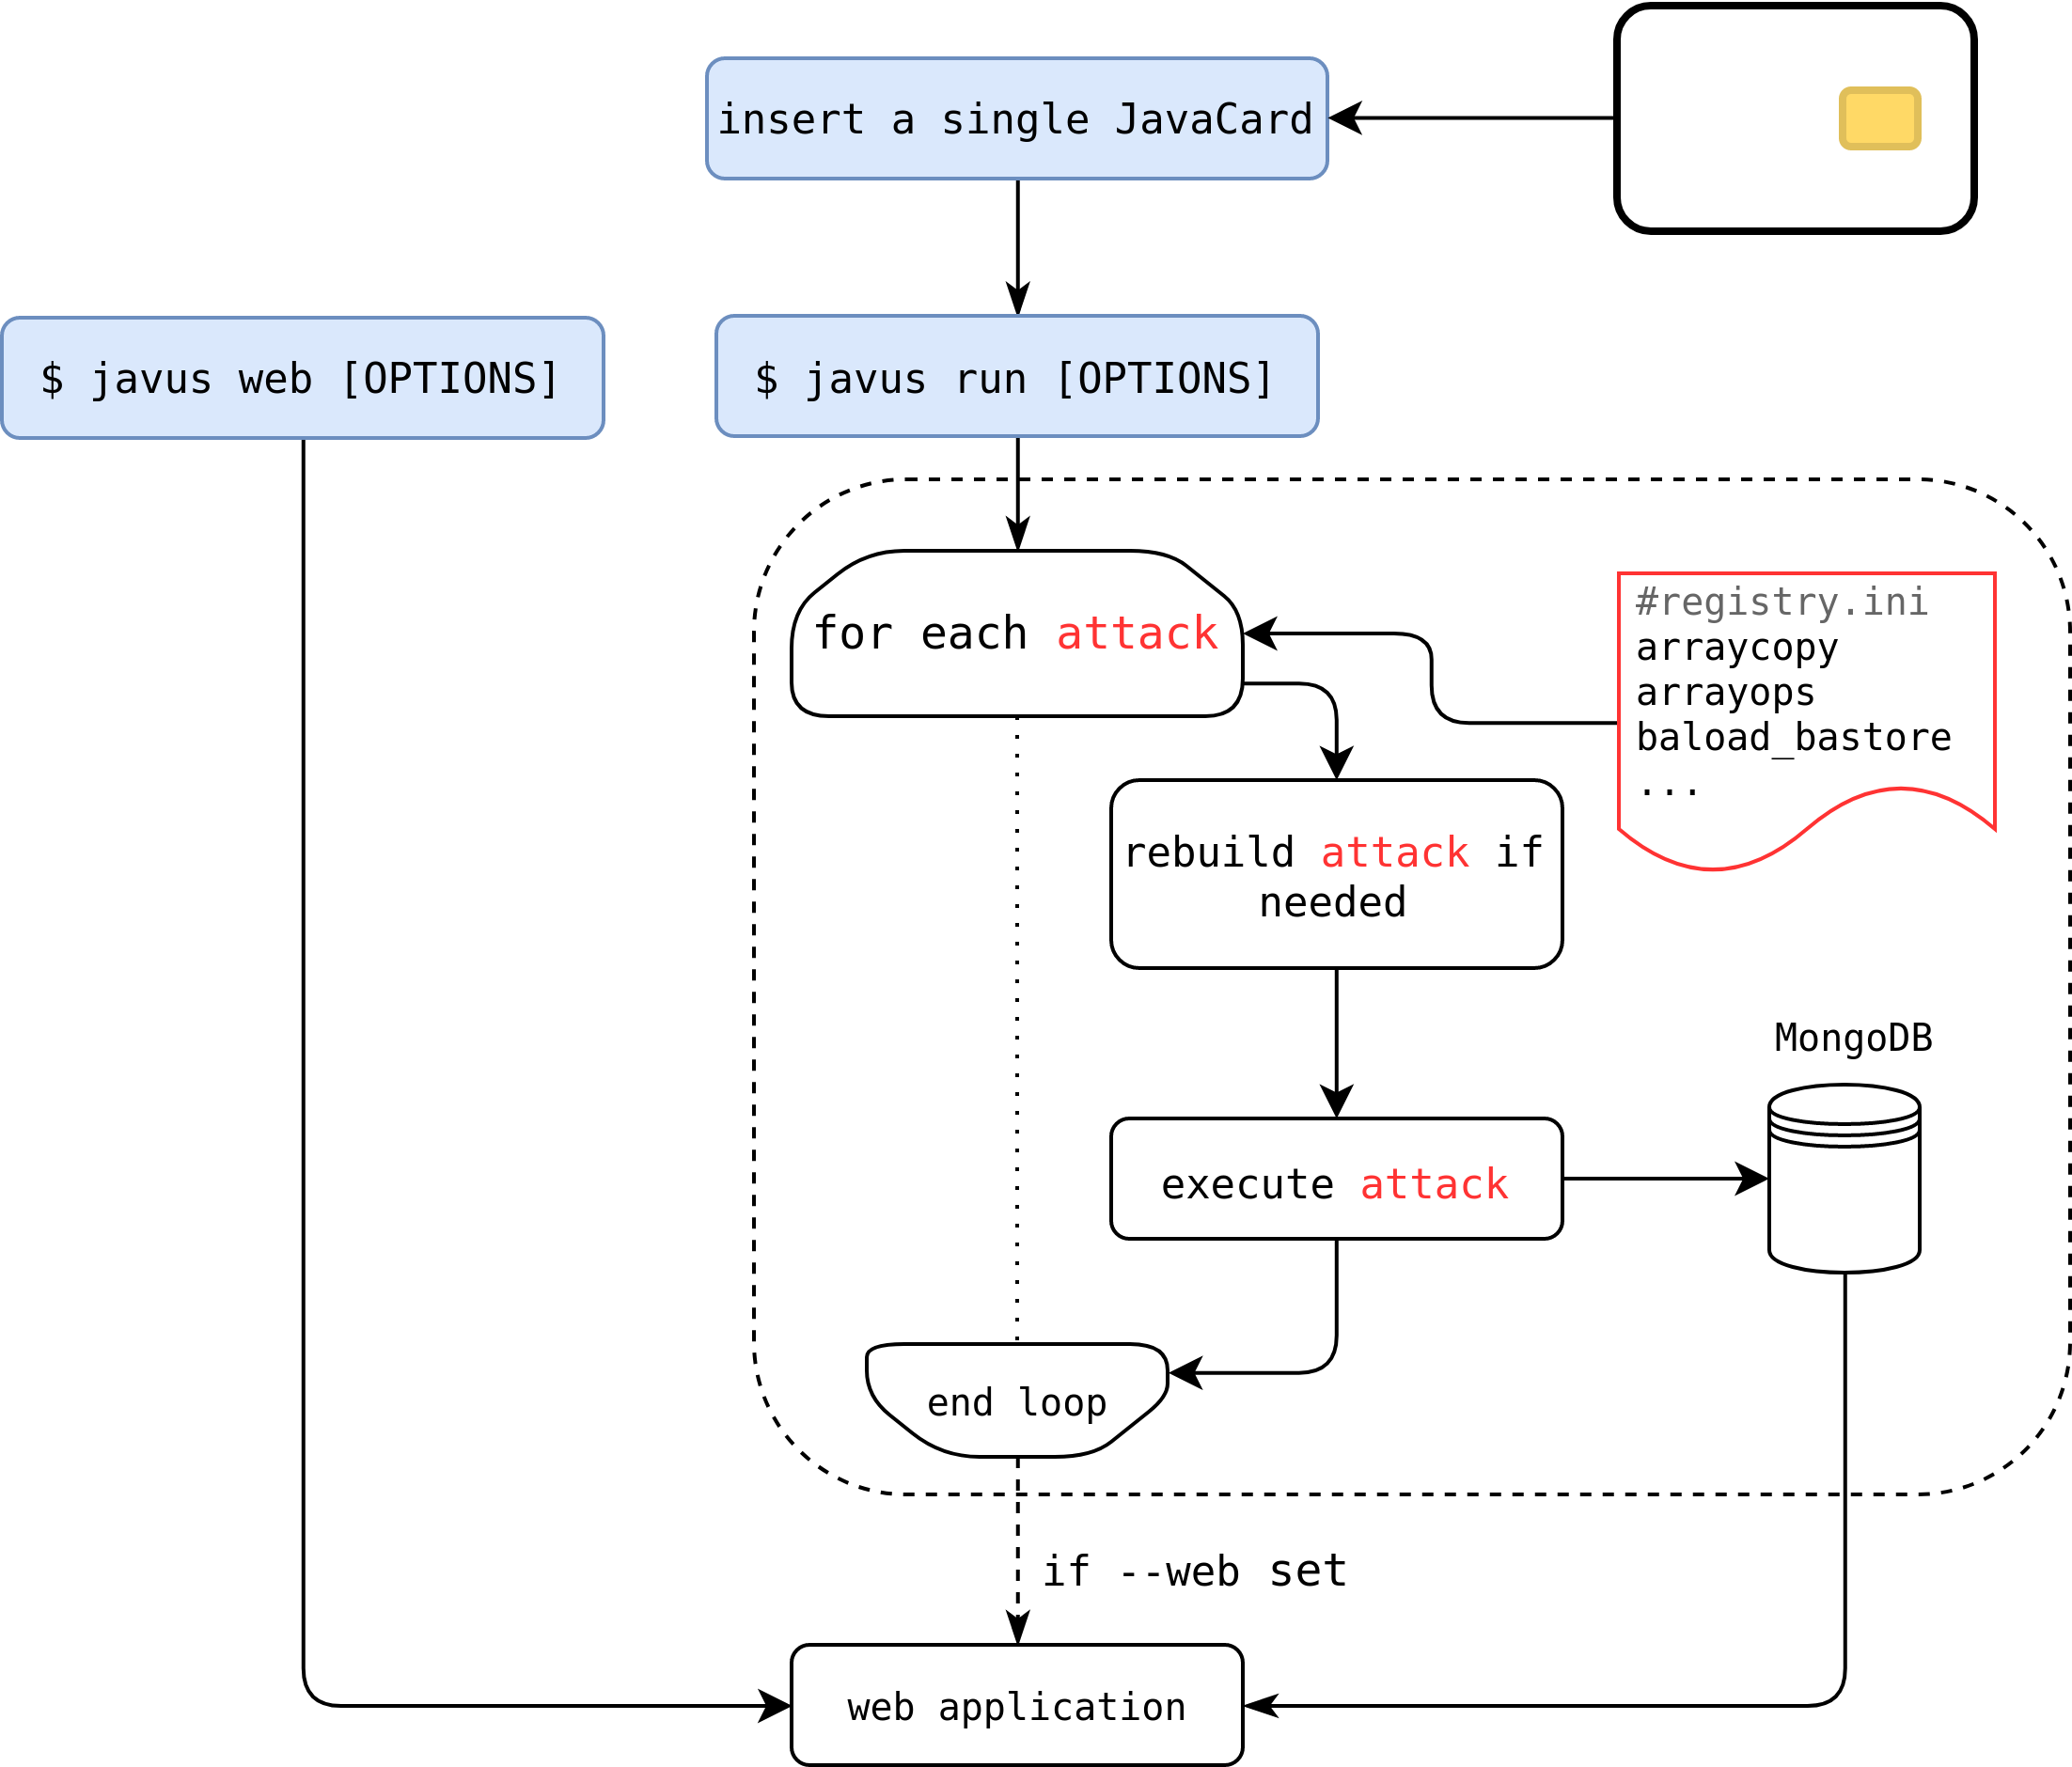
\includegraphics[width=.9\textwidth]{src/diagrams/full-design-new.png}
    \caption{High-level diagram of the run of the testing framework.} % The part with the dashed rectangle is visualized in more detail in the figure~\ref{fig:execute-attack-diagram}.}
        \label{fig:full-design-diagram}
    \end{figure}

        
        % \subsection{The repository structure}
The project is using Git for its version control and it is mainly a Python package. The following paths are relative from the directory \projectroot, which is the root of the Git repository. The Python sources are in \filepath{javus/}, the attacks' source codes are in \filepath{javus/data/attacks/<attack-name>} in respective directories. The file \filepath{javus/data/registry.ini} defines which attacks are enabled. The main command line utility is called \javus. Full Git repository description is in Appendix~\ref{sec:gitrepo}.


        % Now that the reader is familiar with the framework specifications and has overview of the project hierarchy we can go deeper into the internals of the tool. Because the framework takes the advantage of several different tools and integrates them together it was not helpful to follow one particular design pattern. The project is implemented mainly in Python and as such uses the Object Oriented Programming paradigms and also takes the advantage of Python's feature of dynamic imports. Several external tools are used through a \textit{wrapper} class objects, that create internal API (see Appendix~\ref{subsubsec:gpp}).


    \subsection{Building and executing the attacks}\label{sec:build-execute-attacks}

    The figure~\ref{fig:full-design-diagram} shows a single run of the testing tool \javus. The blue boxes represent a user input. The user is only required to insert the JavaCard and execute a single command \javusrun (which invokes the \mintinline{bash}{javus.analyzer.App} class that is responsible for orchestrating the complete analysis). Once the tool is invoked, it loads the registered attacks and executes them one by one. The results are updated to the MonogDB database continuously, because the card can stop working at any time during the run.
    % (as the reader will see in the section~\ref{chp:results}).
    Executing multiple attacks automatically is not\linebreak straightforward.
    % For reasons that are explained later in~\ref{sec:uniq-aid}
    Due to potential AID conflicts of existing applets on the tested JavaCard and those installed during the run we need to have the ability to dynamically rebuild an attack during the run of the framework.
    %Moreover, the way attack applets and packages are built can differ across the spectrum of attacks.

    Not only the build process can differ with each attack, but also the execution --- naturaly, each attack can consist of multiple stages (e.g. installing different number of CAP files, sending various number of APDUs).
    %We will cover this in more detail in~\ref{sec:attack-recipe}, but for now, we will only explain, how per attack build and execution is implemented.

    After \shortappclass handles the command line arguments it hands the execution over to \mintinline{python}{javus.analyzer.AnalysisManager}, which iterates over the registered attacks (loaded from \filepath{registry.ini}). For each attack \mintinline{python}{AnalysisManager} loads the appropriate subclass of \shortbuilderclass respectively \shortexecutorclass that is responsible for building, respectively executing the attack. Each attack is then build for all supported SDK versions and executed on the target JavaCard.

    Eight attacks are currently included in the framework, however, new ones can be added. To do so the actual source code for the attack is needed alongside the different stages defined in a Python module file (see~\cite{anon2020thesis} for details). The framework uses Docker to achieve cross-platformity or can be invoked natively on Linux. The results of the individual runs can be viewed in a simple web application (see figure~\ref{fig:web-interface-pic}).

    \begin{figure}[htb!]
        \centering
        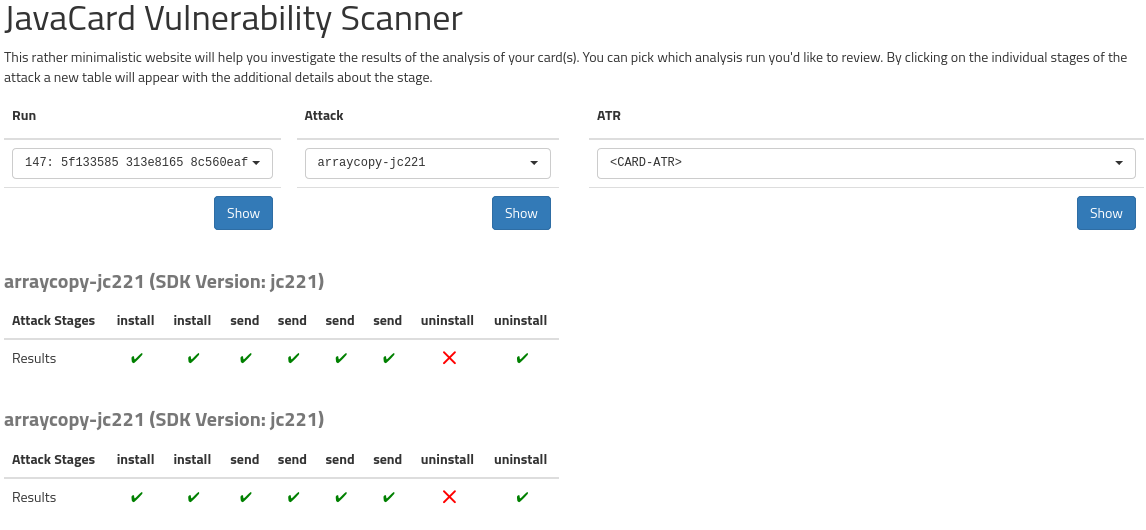
\includegraphics[width=\textwidth]{src/imgs/web-app-all.png}
        \caption{Web interface that allows to filter the results on runs, attacks or cards.\label{fig:web-interface-pic}}
    \end{figure}
    % Now we will take a closer look at those two classes. While reading the next sections the reader can consult the diagram in the figure~\ref{fig:execute-attack-diagram}.
% FIXME sub?
\section{Fuzzing of JavaCards\label{sec:fuzzing}}
While no new attacks have been discovered during the research and implementation of \projectname we have come up with a way of using fuzzing for testing the security of JavaCards. Fuzzing or fuzz testing (for more details see for example \cite{ossfuzz}) is a way of automated testing of binaries, applications, services, etc. Random or semi-random inputs (such as command line invocation strings or files) are generated and then passed to the targetted application. This process easily scales and can be run in parallel. The behaviour of the target application is observed for each random input and usually in case of a crash (or other unexpected output) is noted alongside the input that produced it. This process requires none or very little user interaction.

    % \subsection{Crashcourse in fuzzing}
    \subsection{Fuzzing of JavaCards}
    Fuzzing JavaCards is not as straightforward as fuzzing for example a binary file. \textit{Flooding} a JavaCard with random applets and APDUs will most probably result in the JavaCard getting muted or blocked (such results were observed even for few manually executed and not completely random inputs). However, we have come up with two approaches that allow us to use fuzz testing against the JavaCard platform. First, we will look at fuzzing a real JavaCards. We take a bit more elaborate approach instead of sending completely random inputs to the JavaCard.

    We will start with a working and valid CAP file \texttt{seed.cap}, then create a fuzzed version of that file (for example using~\cite{radamsa}). If this new \texttt{fuzzed.cap} file fails the off-card verification process, we will attempt to install it on a real card. If the card accepts it, it means that the on-card bytecode verifier is not \textit{aligned} with the off-card one. We could also do it the other way around --- if the off-card verifier accepts the \texttt{fuzzed.cap} we will install it and if the on-card verifier reports and error during the installation we have another discrepancy between the verifiers. On the next few lines the reader can see pseudo code of the first fuzzing technique:

    % \subsection{Fuzzing of \cref}

\begin{minted}[linenos]{text}
while true:
    generate a valid CAP file seed.cap
    use fuzzing on seed.cap to generate fuzzed.cap
    verify fuzzed.cap with off-card
    if the verification succeeds:
        continue to line 2
    else:
        try to install fuzzed.cap onto a target JavaCard
        if the installation fails:
            continue to line 2
        else: 
            save the file fuzzed.cap as witness.cap
\end{minted}

Fuzz-testing is usually done continuously (running for days up to months at a time). We have used the previous algorithm to test some of the JavaCards for several hours up to a day. This approach resulted in a few discrepancies found. Those were mostly related to the problem of missing required CAP file components as defined in~\cite{jcspecs31download} --- the off-card verifier reported a missing component (e.g. Descriptor component) while the loading and installation of the CAP file succeeded. Such results are interesting, but do not immediately yield an attack or ways to exploit this issue --- further research in this area is required.

While a way of fuzzing real JavaCards can yield interesting results (testing the actual device is usually preferred over testing just some simulation), it is quite a slow process (compared to fuzzing e.g.\ binaries). And while it can be run in parallel on multiple cards this does not fix the problem of cards getting muted or blocked unexpectedly. The work done by Security Explorations together with our own results (presented in the next section) show that finding issues in the Reference implementation is worth the effort. Therefore we propose another way of testing \cref --- fuzzing it directly.

Reference implementation mimics the usage of a CAD and a JavaCard, but everything is done on a software level. While the actual setup of fuzzing will be a bit different the speed up is expected to be significant. And not only that, because the \cref is a common binary we can take advantage of debugging tools and automatically investigate e.g.\ the \cref memory changes during the fuzz-testing. What we could potentially see are changes in the contexts that do not belong to the currently selected applet. At the moment those are only high-level ideas, but there does not seem to be anything preventing this kind of fuzzing.

\section{The results on real cards and discussion}\label{chp:results}
In this section we will utilize the attacks discussed in the section~\ref{sec:state-of-the-art} and the testing framework JavaCard Vulnerability Scanner presented in the section~\ref{sec:javacard-vulnerability-scanner} and analyze a set of real JavaCards. Aquiring a large number of distinct JavaCards is not an easy task (as they are usually hard to come by in small $< 1000$ quantities), however, we had an interesting variety of JavaCards available for testing. The tested JavaCard were fabricated between the years 2011 a 2017 and the operating systems on these cards were released between the years 2010 and 2018. The list of the cards can be seen in the table ~\ref{tab:card-list}.

\begin{table}[htb]
    \hfill
    \parbox[t][][t]{.45\linewidth}{
        \centering
            \centering
    \begin{tabular}{@{}lllll@{}}
        \toprule
        \textbf{ID\footnotemark} & \textbf{JC Version} & \textbf{Type} & \textbf{GP} \\
        \midrule
        A   & 3.0                & -                & 2.1.1 \\
        B   & 3.0                & EMV              & 2.1.1 \\
        C   & 2.2                & -                & 2.1.1 \\
        C*   & 2.2                & -                & 2.1.1 \\
        D   & 2.2                & EMV              & 2.1.1 \\
        F   & 2.2                & -                & 2.1.1 \\
        G   & 2.2                & -                & -     \\
        H   & 2.2                & -                & 2.1.1 \\
        I   & 2.2                & -                & 2.1.1 \\
        I*   & 2.2                & -                & 2.1.1 \\
        J   & 3.0                & -                & 2.1.1 \\
        \bottomrule
    \end{tabular}
    \caption{%
        List of the cards, that undergone the analysis. The star next to the card ID denotes a different physical card of the same type.
        \label{tab:card-list}
    }

    }
    \hfill
    \parbox[t][][t]{.45\linewidth}{
        \centering
        \begin{tabular}{@{}ll@{}}
            \toprule
                mark & stage result \\
            \midrule
                \passmark & passed \\
                \failmark & failed \\
                \skipmark & skipped\\
            \bottomrule
        \end{tabular}
        \caption{The meaning of the different marks in the following tables.\label{tab:stage-legend}}
    }
    % \end{table}
\end{table}
\footnotetext{The symbol E is missing, because the card got blocked completely during the analysis and renaming could lead to the unwanted mix of the already obtained results.~GP stands for GlobalPlatform~\cite{globalplatform} and the number refers to the version of the specifications the card adheres to.}

    \subsection{Results of the individual attacks}

        The JavaCard Vulnerability Scanner currently tests only attacks, that have been published previously. Nevertheless, during the analysis we have indentified a few cards, which are still vulnerable to some of the attacks. We will continue to study the consequences of those attacks on the affected cards and disclose the results to their respective manufactures if necessary.


    % \section{Results of the individual attacks}
        % Before we dive into the results of particular attacks we will

        % TODO Some cards are doubled explain. Card B is got blocked during the analysis?
        We will often mention for which SDK version we have obtained the results (as they differ significantly). To ease the work for the reader we will not always list all the versions, but write only their range. For that purpose we will use their natural chronological ordering.% (2.1.1. $<$ 2.1.2. $<$ 2.2.1. $<$ 2.2.2. $<$ 3.0.3 $<$ 3.0.4. $)

        We have investigated the behaviour of eleven distinct physical JavaCards and we have performed eight attacks on most of them, therefore we have collected a lot of results. In the following subsections we will cover the two attacks mentioned in the second section. We point out, that when we talk about an attack or stage being \textit{successful} we take the perspective of the adversary and not the defender. The legend for the tables that will be presented is in the table~\ref{tab:stage-legend}.

\setlength{\tabcolsep}{.5pt}
\renewcommand{\arraystretch}{.20}
\setlength{\floatsep}{0pt}

\begin{table}[htb!]
    \captionsetup{font=footnotesize}
    \parbox[b][][b]{.45\linewidth}{
        	\footnotesize
	\centering
	\begin{tabular}{@{}llcccccccc@{}}
\toprule
\textbf{card}	&	\textbf{SDK}	&	{\small \texttt{\rot{\textbf{install}}} }	&	{\small \texttt{\rot{\textbf{install}}} }	&	{\small \texttt{\rot{\textbf{READ MEM}}} }	&	{\small \texttt{\rot{\textbf{WRITE MEM}}} }	&	{\small \texttt{\rot{\textbf{WRITE MEM}}} }	&	{\small \texttt{\rot{\textbf{READ MEM}}} }	&	{\small \texttt{\rot{\textbf{uninstall}}} }	&	{\small \texttt{\rot{\textbf{uninstall}}} }\\
\midrule
A	&	3.0.4	&	\passmark	&	\passmark	&	\failmark	&	\failmark	&	\failmark	&	\failmark	&	\failmark	&	\failmark\\
C	&	3.0.5u3	&	\failmark	&	\skipmark	&	\skipmark	&	\skipmark	&	\skipmark	&	\skipmark	&	\skipmark\\
C*	&	3.0.5u3	&	\failmark	&	\skipmark	&	\skipmark	&	\skipmark	&	\skipmark	&	\skipmark	&	\skipmark\\
D	&	2.2.1	&	\passmark	&	\passmark	&	\failmark	&	\failmark	&	\failmark	&	\failmark	&	\failmark	&	\failmark\\
F	&	3.0.5u3	&	\failmark	&	\skipmark	&	\skipmark	&	\skipmark	&	\skipmark	&	\skipmark	&	\skipmark\\
G	&	3.0.5u3	&	\failmark	&	\skipmark	&	\skipmark	&	\skipmark	&	\skipmark	&	\skipmark	&	\skipmark\\
H	&	3.0.5u3	&	\failmark	&	\skipmark	&	\skipmark	&	\skipmark	&	\skipmark	&	\skipmark	&	\skipmark\\
I	&	3.0.5u3	&	\failmark	&	\skipmark	&	\skipmark	&	\skipmark	&	\skipmark	&	\skipmark	&	\skipmark\\
I*	&	3.0.5u3	&	\failmark	&	\skipmark	&	\skipmark	&	\skipmark	&	\skipmark	&	\skipmark	&	\skipmark\\
J	&	3.0.4	&	\passmark	&	\passmark	&	\passmark	&	\passmark	&	\passmark	&	\passmark	&	\failmark	&	\passmark\\
\bottomrule
\end{tabular}
\caption{The best results across cards and SDKs for \texttt{arraycopy}.}
\label{tab:best-arraycopy}

    }
    \hfill
    \parbox[b][][b]{.45\linewidth}{
        % 	\footnotesize
	\centering
	\begin{tabular}{@{}llcccccccccc@{}}
\toprule
\textbf{card}	&	\textbf{SDK}	&	{\small \texttt{\rot{\textbf{install}}} }	&	{\small \texttt{\rot{\textbf{install}}} }	&	{\small \texttt{\rot{\textbf{READ MEM}}} }	&	{\small \texttt{\rot{\textbf{WRITE MEM}}} }	&	{\small \texttt{\rot{\textbf{WRITE MEM}}} }	&	{\small \texttt{\rot{\textbf{WRITE MEM}}} }	&	{\small \texttt{\rot{\textbf{WRITE MEM}}} }	&	{\small \texttt{\rot{\textbf{READ MEM}}} }	&	{\small \texttt{\rot{\textbf{uninstall}}} }	&	{\small \texttt{\rot{\textbf{uninstall}}} }\\
\midrule
A	&	3.0.5u3	&	\passmark	&	\failmark	&	\skipmark	&	\skipmark	&	\skipmark	&	\skipmark	&	\skipmark	&	\skipmark	&	\skipmark	&	\passmark\\
C	&	3.0.5u3	&	\failmark	&	\skipmark	&	\skipmark	&	\skipmark	&	\skipmark	&	\skipmark	&	\skipmark	&	\skipmark	&	\skipmark\\
C*	&	3.0.5u3	&	\failmark	&	\skipmark	&	\skipmark	&	\skipmark	&	\skipmark	&	\skipmark	&	\skipmark	&	\skipmark	&	\skipmark\\
D	&	3.0.5u3	&	\passmark	&	\failmark	&	\skipmark	&	\skipmark	&	\skipmark	&	\skipmark	&	\skipmark	&	\skipmark	&	\skipmark	&	\passmark\\
F	&	3.0.5u3	&	\failmark	&	\skipmark	&	\skipmark	&	\skipmark	&	\skipmark	&	\skipmark	&	\skipmark	&	\skipmark	&	\skipmark\\
G	&	3.0.5u3	&	\failmark	&	\skipmark	&	\skipmark	&	\skipmark	&	\skipmark	&	\skipmark	&	\skipmark	&	\skipmark	&	\skipmark\\
H	&	3.0.5u3	&	\failmark	&	\skipmark	&	\skipmark	&	\skipmark	&	\skipmark	&	\skipmark	&	\skipmark	&	\skipmark	&	\skipmark\\
I	&	3.0.5u3	&	\failmark	&	\skipmark	&	\skipmark	&	\skipmark	&	\skipmark	&	\skipmark	&	\skipmark	&	\skipmark	&	\skipmark\\
I*	&	3.0.5u3	&	\failmark	&	\skipmark	&	\skipmark	&	\skipmark	&	\skipmark	&	\skipmark	&	\skipmark	&	\skipmark	&	\skipmark\\
J	&	3.0.5u3	&	\passmark	&	\failmark	&	\skipmark	&	\skipmark	&	\skipmark	&	\skipmark	&	\skipmark	&	\skipmark	&	\skipmark	&	\passmark\\
\bottomrule
\end{tabular}
% \caption{\texttt{arrayops}}
\caption{The best results across cards and SDKs for \texttt{arrayops}.}
\label{tab:best-arrayops}

        	\footnotesize
	\centering
	\begin{tabular}{@{}llccccc@{}}
\toprule
\textbf{card}	&	\textbf{SDK}	&	{\small \texttt{\rot{\textbf{install}}} }	&	{\small \texttt{\rot{\textbf{install}}} }	&	{\small \texttt{\rot{\textbf{TRIGGER_SWAPX}}} }	&	{\small \texttt{\rot{\textbf{uninstall}}} }	&	{\small \texttt{\rot{\textbf{uninstall}}} }\\
\midrule
A	&	2.2.1	&	\passmark	&	\passmark	&	\failmark	&	\failmark	&	\failmark\\
C	&	3.0.5u3	&	\failmark	&	\skipmark	&	\skipmark	&	\skipmark\\
C*	&	3.0.5u3	&	\passmark	&	\failmark	&	\skipmark	&	\skipmark	&	\passmark\\
D	&	2.2.1	&	\passmark	&	\passmark	&	\failmark	&	\passmark	&	\passmark\\
F	&	2.2.2	&	\passmark	&	\passmark	&	\passmark	&	\passmark	&	\passmark\\
G	&	3.0.5u3	&	\failmark	&	\skipmark	&	\skipmark	&	\skipmark\\
H	&	2.2.2	&	\passmark	&	\passmark	&	\passmark	&	\passmark	&	\passmark\\
I	&	3.0.5u3	&	\failmark	&	\skipmark	&	\skipmark	&	\skipmark\\
I*	&	2.2.1	&	\passmark	&	\passmark	&	\passmark	&	\passmark	&	\passmark\\
J	&	2.2.1	&	\passmark	&	\passmark	&	\passmark	&	\passmark	&	\passmark\\
\bottomrule
\end{tabular}
% \caption{\texttt{swap_x}}
\caption{The best results across cards and SDKs for \texttt{swap_x}.}
\label{tab:best-swap_x}

    }
\end{table}

\subsection{Results of \texttt{arraycopy}}\label{subsec:result-arraycopy}
            As the reader can see in the table~\ref{tab:best-arraycopy} only a single card was vulnerable to this attack. For every SDK version the cards \Cnewcard, \Fcard, \Gcard, \Hcard, \Inewcard prevented already the load of the malicious CAP \vulnscap. Each responded with the status word \swwrongdata, except the \Cnewcard, which has failed with \swunknown and \Inewcard with \swwrongdata. The \vulnscap could not have been installed on \Icard, \Ccard and the status word \swconditionsnotsatisfied was returned.
            % \Inewcard also acted unlike \Icard with the load failing with \mintinline{bash}{0x6A80 - WRONG_DATA}.
            % \import{src/tables/subtables}{best-arraycopy.tex}
            % FIXME card stopped working 97 JCRE muteing card

            However, not all cards have failed the installation of \vulnscap. With SDK 2.2.1 the card \Dcard let both CAP files be installed, but returned \swclanotsupported when selecting applet to execute the first send stage. Then, during the execution of the first send stage the card stopped working with the error \scardenottransacted. After several minutes the card started to work again and both applets could be deleted with GlobalPlatformPro using the \mintinline{bash}{--delete} flag.

            For the SDK versions 3.0.5u1, 3.0.5.u2 and 3.0.5u3 the card \Acard did fail with \swwrongdata when loading the \appletscap, but for 2.2.1.--3.0.4. SDKs everything was loaded and installed properly, but the send stages failed with \swunknown. Neither of the applets could be uninstalled afterwards and the uninstall command returns \swconditionsnotsatisfied.

            Finally, the most interesting behaviour was obtained with the card \Jcard. For SDKs 3.0.5u1, 3.0.5u2, 3.0.5u3 the load of the file \appletscap failed with \jerror. But for the rest of the SDKs the attack succeeded. All of the send stages passed and the only issue was to uninstall the \appletscap file --- the uninstallation failed with \swconditionsnotsatisfied. Therefore multiple invocation can fill the JavaCards memory and prevent further installations. However, the attack works and according to~\cite{se:oracle:part1} it should allow arbitrary read and write access.


            % The worst of all the cards is the card \Jcard. 
            %Anew
            %Ended same
            %    Anew-jc221
            %    Anew-jc222
            %    Anew-jc303
            %    Anew-jc304
            %    all install succeeded
            %    both applets are installed, however, cannot be uninstalled.
            %    all sends ended with 6f00 - no SW_UKNOWN, no precise diagnosis
            %    all uninstalls failed with 6985, SW_CONDITIONS_NOT_SATISFIED

            %Ended same
            %    Anew-jc305u1
            %    Anew-jc305u2
            %    Anew-jc305u3
            %    applets.cap cannot be install
            %        LOAD failed: 0x6A80 (Wrong data/incorrect values in data)
            %    however, uninstalling the vulns.new.cap can be uninstalled

            %%D - TODO failed during jc221
            %%E - TODO
            %F - all same
            %    LOAD failed: 0x6A80 (Wrong data/incorrect values in data)
            %G - all same
            %    LOAD failed: 0x6A80 (Wrong data/incorrect values in data
            %H - all same
            %    LOAD failed: 0x6A80 (Wrong data/incorrect values in data

            %I - all same
            %    INSTALL [for load] failed: 0x6985 (Conditions of use not satisfied
            %C for all sdks the vulns.new.cap cannot be installed
            %    INSTALL [for load] failed: 0x6985 (Conditions of use not satisfied)

            %Cnew for all sdks the vulns.new.cap cannot be installed
            %    LOAD failed: 0x6F00

            %Inew - all same LOAD failed: 0x6A80 (Wrong data/incorrect values in data
            %J
            %    most different applets.cap
            %    jc221,jc222,jc303,jc304 - DELETE failed: 0x6985 (Conditions of use not satisfied)
%jc305u1 jc305u2 jc305u3 - LOAD failed: 0x6438 applets.cap

            % C all vulns.new.cap  INSTALL [for load] failed: 0x6985 (Conditions of use not satisfied
            % Cnew all vulns.new.cap load failed with 0x6f00


            % B, E no results
            % F all vulns.new.cap  LOAD failed: 0x6A80 (Wrong data/incorrect values in data
            % G all vulns.new.cap  LOAD failed: 0x6A80 (Wrong data/incorrect values in data
            % H all vulns.new.cap  LOAD failed: 0x6A80 (Wrong data/incorrect values in data
            % Inew all applets.cap LOAD failed: 0x6A80 (Wrong data/incorrect values in data

            % I all applets.cap INSTALL [for load] failed: 0x6985 (Conditions of use not satisfied

            % Anew  all applets.cap load failed wih 0x6A80 swwrongdata, vulns.new.cap uninstall ok
            % D all applets.cap  LOAD failed: 0x6A80 (Wrong data/incorrect values in data

            % J all vulns.new.cap LOAD failed: 0x6438

            % \import{src/tables/subtables}{best-arrayops.tex}

            % FIXME use attack that had better results

            % \subsection{\texttt{arrayops}}
            % % TODO figure out, where is this frooom
            % This attack can only be built for the 3.0.5u1--3.0.5u3 SDK versions. The results of the attack do differ across the range of the cards (see the table~\ref{tab:best-arrayops}), however, for fixed card the results don't differ across the SDKs.
            
            % The load of \vulnscap failed with the status word \shortswwrongdata for the cards \Fcard, \Gcard, \Hcard and \Inewcard with status word \shortswunknown for \Cnewcard card. For \Jcard the loading of \vulnscap returned unknown status word \mintinline{python}{0x6438}. The card \Ccard could not install \vulnscap and gave \shortswconditionsnotsatisfied error. 

            % The cards \Acard and \Dcard allowed the installation of \vulnscap, but returned \shortswwrongdata during the load of \appletscap. The card \Icard exited the installation of \appletscap with \shortswconditionsnotsatisfied.
            % Therefore, none of the tested cards are vulnerable to this kind of attack.

        \subsection{Results of \texttt{swap_x}}\label{subsec:swapx}
        % TODO add \xspace to the custom mintinlines

            Four cards allowed all attack stages as the reader can see in the table~\ref{tab:best-swap_x}.
        % TODO align the card an SDK to the top in the table?
            % \import{src/tables/subtables}{best-swap-x.tex}
            The card \Gcard prevented the loading of \vulnscap for all SDKs and returned the unknown status word \mintinline{python}{0x6484}. For the cards \Ccard and \Icard the attack got a bit further and failed during the installation of \vulnscap with the error \shortswconditionsnotsatisfied, regardless of the SDK.

%TODO TRIGGER_SWAPX did overflow, fix, breaklines and breakafter did not work
            Again, the \Cnewcard (for all SDKs) behaved differently and let the \vulnscap to be installed, but failed during the loading of \appletscap and gave \shortswconditionsnotsatisfied. The card \Acard installed both applets successfully for SDK 2.2.1., but while sending the \mintinline{python}{TRIGGER_SWAPX} the card stopped working with \scardwunpoweredcard. Other SDKs were not tested.

        The card \Dcard could not load the \appletscap for SDKs 2.2.2--3.0.5u1 and returned the status word \shortswwrongdata, moreover, for 3.0.5u1 the card stopped working with \scardenottransacted. Only for the SDK 2.2.1. both applets were installed and the attack failed during the execution of the send stage with \shortswclanotsupported.


    Now we are moving on to the cards, that could not prevent the attack completely. As observed previously, the cards \Fcard and \Hcard behaved in the exact same way. For the SDKs 3.0.3.--3.0.5u3 the loading of \appletscap failed with \shortswwrongdata, however, the for other versions 2.2.1. and 2.2.2. the attack worked completely. The card \Inewcard did react only slightly differently. The attack has succeeded for SDK 2.2.2. and failed for the rest while loading the \appletscap, but this time the returned status word was \shortswconditionsnotsatisfied.

    Finally, the situation with the \Jcard. Again, the oldest SDK version 2.2.1. did allow the attack to pass all of the stages. For the SDK versions 2.2.2.--3.0.4. both applets were installed, but the send staged resulted in the error word \shortswinsnotsupported. For the rest of the SDKs 3.0.5u1--3.0.5u3 the attack did not go further than installing the \vulnscap and failed during the loading of \appletscap with the unknown status word \mintinline{python}{0x6438}.


            \subsection{Overall results}

        To give the reader an overview across all the cards and all the attacks we present them in a single table~\ref{tab:results-overview}. The SDK version in the table represents the newest SDK for which the given attack POC has worked. What is reassuring is the fact, that the currently oldest attack registered in JavaCard Vulnerabilty Scanner the \texttt{transaction_confusion} did not work on any of the cards. However, the card J even though it is only few years old was vulnerable to three out of eight attacks.
    
        We plan to further look into the attacks to see, if they can used to retrieve and alter different memory regions as is suggested in~\cite{se:oracle:part1}.

\setlength{\tabcolsep}{2pt}
\renewcommand{\arraystretch}{1.2}

    \import{src/tables/subtables}{results-overview.tex}

\setlength{\tabcolsep}{\oldtabcolsep}
\renewcommand{\arraystretch}{1.2}
\setlength{\floatsep}{\oldtabcolsep}


\section{Conclusion}

        % In the very last section we will take a moment to reflect on the JavaCard Vulnerability Scanner framework and try to have a peek into its future. Then we will close off this text with the summary of the security of JavaCard Virtual Machine.

        % \subsection{The future of JavaCard Vulnerability Scanner}

        As observed in the previous results and in our own as well it is apparent that different JavaCards implement the on-card bytecode verifiers and run-time checks differently. This is not surprising, considering that the complete JavaCard RE is left to the JavaCard vendors to be implemented and already~\cite{Mostowski07testingthe} showed that the specifications are not always followed completely or can be ambiguous.
        % Since some cards perform better it suggests that the vendors could learn from each other in order to improve the JavaCard platformi
        % From this perspective we see potential in a project like JavaCard Vulnerability Scanner that could help bringing more transparency into the security of JavaCards. Our tool is capable to test a JavaCard across various SDKs and attacks and can gather results similar to~\ref{tab:results-overview}.
        We see potential in a project like JavaCard Vulnerability Scanner, because it can help to bring more transparency into the security of JavaCards. Our tool is capable of testing a JavaCard across various SDKs and attacks and can gather results similar to the ones in the table~\ref{tab:results-overview}. Moreover, the web application can be made public and therefore researches could share the results. We invite other developers and researchers to use this tool locally, find its shortcomings or opportunities for new features and submit both at \url{\githuburl} (incomplete URL due to anonymization). 
        % As stated previously, the JavaCard Vulnerability Scanner is still a prototype. It can serve as a base for future analysis of JavaCards, because it can be already used for executing regular applets and not only testing logical attacks. The implementation was done in such a way that it allows to switch different parts or extend another one. In case the JavaCard community will find JavaCard Vulnerability Scanner useful the web application can be moved into a separate project and be hosted as a public service that would allow not only researchers to submit or verify their own results from JavaCard Vulnerability Scanner. Such public database could speed up the development of the security of the JavaCard Virtual Machine JavaCard Runtime Environment and also help to make the applications developed for this platform overall more secure.

        % For now, however, we invite other developers and researchers to use this tool locally, find its shortcomings or opportunities for new features and submit both at \url{\githuburl}. It would only be for the better if academic results would affect the non-academic world and vice-versa. Tools developed just for the sake of satisfying formal academic requirements are bound to die out quickly.
        % We invite other developers and researchers to use this tool locally, find its shortcomings or opportunities for new features and submit both at \url{\githuburl}. 
        % It would only be for the better if academic results would affect the non-academic world and vice-versa. Tools developed just for the sake of satisfying formal academic requirements are bound to die out quickly.

        % According to Oracle~\cite{oraclehome} more than 9 billion JavaCard enabled devices have been shipped since 1998 and the number keeps rising. For several years it is possible to buy open JavaCard that allow installation of new custom applets and therefore we can expect more applications emerging on the JavaCard platform.
        % JavaCard platform and the its development still kept propriatery.
        % However, it is a platform deployed all over the world in billions of units and this number keeps raising.
        % And as examples from other fields of information technology show, there will hardly ever come a struggle to have a particular platform \textit{too much secure}. Rather, every step into making the security assessment of a given platform simpler to perform and more thorough is welcomed. The author would be honoured, if this tool would help to pave the way alongside the projects like JCAlgTest and ECTester (and other), towards more transparent and secure JavaCard platform.

        % \subsection{Possibilities for future attacks}

        % Throughout the many attacks the reocurring problem is type confusion or insufficient type checking. What is often mentioned when discussing additional run-time checks are the limited resources of JavaCard. However, as observed in~\cite{se:oracle:part1,se:oracle:part2,se:oracle:part3} the input value checking is not done for \textit{some} methods properly even in \texttt{cref}. The reference implementation is not limited in its resources as it can run on a regular computer. Testing on real JavaCards is not much cost effective, as the JavaCards can get damaged, blocked, locked or render unsuable in other way beyond repair. It happened to us during the development of \javus for at least three JavaCards. On one hand, we have developed JavaCard Vulnerability Scanner to bring testing to \textit{real} JavaCards to bigger audience and to gather results from more JavaCards than individual researchers is able. Testing is often most helpful on the real system. On the other hand, due to the cost effectivness it is good to see that vulnerabilities discovered in the reference implementation do affect real JavaCard and therefore the analysis does help to improve the overall security of the platform.


        % The vulnerabilites presented in~\ref{sec:related-work} are often elaborate as is visible from the common step of CAP file alteration or first discovering e.g. array metadata and consequently using them in later stages of the attack. We do not know, what was the approach of Security Explorations, that they discovered so many vulnerabilites, maybe they have used more automated and therefore possible thorough anlaysis of \texttt{cref}. Nevertheless, using \texttt{cref} for analysis brings fruits.


        % Further, our approach~\ref{subsec:onofffuzzing} to on-card vs. off-card BCV fuzzing has yield preliminary results. We have not seen fuzzing used for testing JavaCard security. At first sight JavaCard does not seem to be a great platform for fuzz testing, because it relies on generating and analyzing huge number of inputs/outputs to the targetted program. We have observed, that the part of current implementation of JavaCard Vulnerability Scanner responsible for communicating with JavaCard is the bottleneck. Fuzz testing can be done in the way it was proposed in~\ref{subsec:onofffuzzing}, but it is expected to be slow. The author thinks, that maybe the whole process could be sped up significantly by first fuzzing the JavaCard RE Reference Implementation and use only subset of those inputs then on real JavaCards. Generating interesting inputs to such fuzz testing could be hard, because the reference implementation can just keep failing due to completely random inputs, but the analysis of the crash can be more elaborate than simply noting a crash of an application (as it is often enough for other fuzz testing). Because \texttt{cref} is started as a process on a standard computer an elaborate monitoring techniques could be used --- the reeader can imagine \textit{fuzzing} \texttt{cref} and making snapshots of the memory after each run. The differences between the snapshots could yield which inputs are more probably to cause a real issue. The input to fuzz testing can be fixed in the bytes regarding the installation of some applet and only subsequent APDUs can be fuzzed.         % from the many attacks, that we have studied we see few take-aways. it is a positive news, that none of the tested cards were vulnerable to the old attack \texttt{transaction_confusion}~\cite{}.

        % % However, the attack was using type confusion and several new vulnerabilites exploiting slightly different type confusion on the level of bytecode instructions and API methods have been discovered recently (little more than a year ago~\cite{se:gemalto:part1, se:gemalto:part

\newpage
\bibliography{./src/sources.bib}
\bibliographystyle{llncs/splncs04}

\end{document}
